\section{Time Petri Nets}
	\label{subsec:redes_con_tiempo}
	In this nets, each transition has an associated interval $[a , b]$ which represents the	possible 
	duration of the activity modeled by the transition.	
	
	\subsection{Mathematical Definition}
		A \emph{Marked Time Petri Net}\cite{garcia_izquierdo}, is mathematically defined as a 8-tuple as follows:
		\begin{equation*}
			PN = \{P, T, I^-, I^+, H,C, m_0, IS\}
		\end{equation*}
		Where,
		\begin{itemize}
			\item \textbf{P} is a non-empty finite set of places.
			\item \textbf{T} is a non-empty finite set of transitions; 
			\begin{equation*}
			P\cap T=\oslash
			\end{equation*}
			\item \textbf{$I^+$}, \textbf{$I^-$} are the possitive and negative incidence matrices.
				\begin{equation*}
					P�T\rightarrow \mathbb{Z}
				\end{equation*}
			\item \textbf{H} is the inhibitors arcs matrix.
				\begin{equation*}
				P�T\rightarrow\{0,1\}
				\end{equation*}
			\item \textbf{C}: is a vector containing the values that represent the maximum amount of 
							tokens that each place of the net can hold.
				\begin{equation*}
				C\rightarrow\mathbb{N}
				\end{equation*}				
			\item $\boldsymbol{m_0}$ is the net initial marking.
				\begin{equation*}
				P\rightarrow \mathbb{N}
				\end{equation*}
			\item \textbf{IS} is the set of static intervals associated with each transition. 
				\begin{equation*}
				T\rightarrow \mathbb{Q}^+ � (\mathbb{Q}^+ \cup \infty)
				\end{equation*}
		\end{itemize}
			
		The \textbf{\emph{IS}} function associates to each transition a pair of values representing
		the minimun and maximum time limits between which the transition may be triggered. In a way 
		that $IS(t) = [min,max]$. Where, $t$ is a transition included in the $T$ set.
		
		As the $IS$ function represents a time interval must meet the following conditions.\\
		\begin{itemize}
			\item $0 	\leq 	min	<	\infty$
			\item $0 	\leq 	max	\leq 	\infty$
			\item $min	\leq 	max \text{ if } max \neq \infty$
			\item $min	< max \text{ if } max   =	 \infty$\\
		\end{itemize}
		
		The value $min$ is called \textbf{Earliest Firing Time (EFT)}. And, the value $max$ is known
		as \textbf{Latest Firing Time (LFT)}.\\
				
		There are two remarkable interval types:
		
		\begin{itemize}
			\item \emph{Intervalo puntual}
				\begin{equation*}
					[\alpha,\alpha]
				\end{equation*}
				In this case, the sensibilization time is fixed. After the time indicated by $\alpha$ 
				the transition has to be fired. An inmediate firing is represented by $\alpha=0$.
			\item \emph{Interval without temporal restriction}\\
				\begin{equation*}
					[0,\infty]			
				\end{equation*}
				The transition has no temporal restrictions to be fired, it will be fired sometime 
				after been enabled.
			\end{itemize}
		
	\subsection{Time Petri Nets States}
			
		In these Petri Nets, the net state is defined by the marking vector ($m$) and an 
		\emph{interval} vector that indicates the time stamp of each trasition. Therefore the net 
		state is:
		\begin{equation*}
			S = (m_0,timer)
			\label{eq:time_net_state}
		\end{equation*}
		 
		
			
	\subsection{Sensitization of the Transitions and Firing Rules}
	\label{subsec:sensitization_transitions}	
		When we refer to transitions, we have to establish the difference between an enabled or 
		sensitized transition, a not enabled or sensitized transition and the firing of a transition.
		
		In a Marked Petri Net whose current mark is $m_k$, we say that transition $t_j$ is enabled 
		or sensitized if and only if $timer_t=0$ and the amount of tokens in all places $p_i$ 
		belonging to these  $\bullet t_j$ is at least equal to the weight of the arc that connects 
		them with the transition $t_j(w(p_i,t_j))$. Mathematically:
		\begin{equation*}
			p_i\in \bullet t_i,m(p_j) \geq w(p_i,t_j)
		\end{equation*}
		If the transition time is zero, $timer_t$ must be enabled to auto-increment with time.
		The sensitized transitions can be fired in the interval [a, b], and his shot causes a new 
		marking, its mean a change of state.
		
		Sensitized transitions can be fired and every time the firing of a transition is completed 
		it generates a new marking for the Petri Net. This means that the net changes its state.
		
		The equation to calculate the new state or new marking reached by the firing of $t_j$ is
		$\delta(m_k,t_j)$, and it is defined as (\ref{eq:new_state_eq}):\\
		
		\begin{equation}
			\delta (m_k,t_j)=
					\begin{cases} 
						m_{k+1} (p_i)=m_k (p_i )-W_{ij} & \forall p_i \in \bullet t_j 
						\\
						m_{k+1} (p_i)=m_k (p_i )+W_{ij} & \forall p_i \in t_j \bullet
						\\
						min \leq timer_{(t_j)} \leq max & 
						\\
						m_{k+1} (p_i)=m_k(p_i) & \mbox{in the rest}
						\\
						 & \mbox{of the cases}
					\end{cases}
				\label{eq:new_state_eq}
		\end{equation}		
				\begin{center}
				$min=a, max=b;$
				\end{center}
		$timer_{(t_j)}$ is incremented in every clock cycle after the transition have been sensitized. 
		
%TODO translate this
	\subsection{Interpretation of the firing of transitions in the system}
		The figure \ref{fig:reactive_systems} represents a reactive systems that responds to events which
		come from the environment, it interacs with the environment. Those events are directed to the Time
		Petri Nets processor.
	
		The responsibility of the processor is arrange events  according to system constraints. These
		constraints are modeled by the Time Petri Net which is used to program the processor. On the
		other hand, multicore system threads also generate events (to request resources, to synchronize) 
		that are directed to the processor.		
		
		\begin{figure}[h]
			\centering
			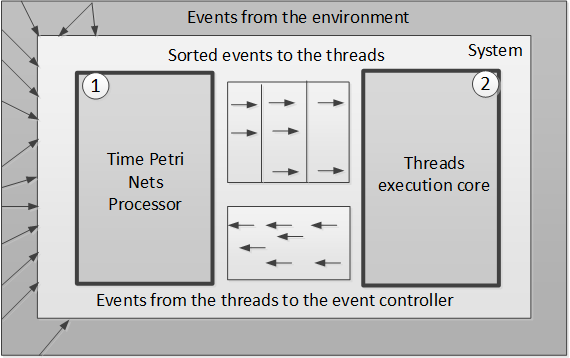
\includegraphics[width=0.85\linewidth]{reactive_system}
			\caption{Reactive systems}
			\label{fig:reactive_systems}
		\end{figure}
		
		Module 1 from the Figure \ref{fig:reactive_systems} receive unsorted events from the environment
		and from the system itself. After the sorting of the events the Time Petri Nets processor
		transmits the result to the threads execution cores (module 2) of the system and the propers
		actions are taken\cite{peterson}. 
		
		In our system the fulfillment of program conditions is associated to sensitized transitions, 
		the resolution of a shot represents the fulfillment of those restrictions and if we associate 
		the request for verification of the conditions to a shot request, the resolution of a shot 
		communicates that conditions have been met.
		
		Definition: conditions for firing a transition from Time Petri Process:
		\begin{enumerate}
			\item The transition must comply with sensitization conditions named in Section
				\ref{subsec:sensitization_transitions}.
			\item The shot must be explicitly communicated by the processes or implicitly 
					recorded in the automatic shots module.
			\item Since it is possible that multiple transitions simultaneously satisfy the conditions
				described in paragraphs 1 and 2, the Time Petri Nets processor will execute first the
				firing with higher priority.\\
		\end{enumerate}	

		Figure \ref{fig:conection_multicore_system} show us how the Time Petri Nets processor is conected
		in a multicore system.
	
		In case that the firing of the transition can not be resolve, it is queued in the input queue, as
		shown in Figure \ref{fig:conection_multicore_system}, until the conditions of the system allow
		its resolution. The solution of the firing is notified to threads through the system bus, using
		the output queue. The threads of the system will execute the proper actions as indicated by 
		the firings that have been resolved, since the resolution of the firings depends on the Time 
		Petri Nets Processor state, which itself represents the state of the system.
	
		\begin{figure}[h]
			\centering
			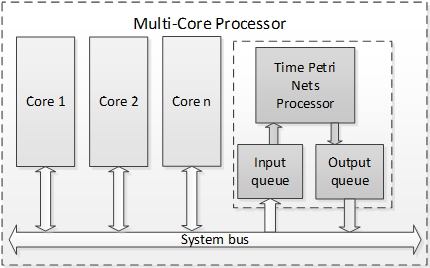
\includegraphics[width=.95\linewidth]{conection_multicore_system}
			\caption{Multicore system with Time Petri Nets processor}
			\label{fig:conection_multicore_system}
		\end{figure}		


